\cleardoublepage
\chapter{Results}
\label{ch:results}
\label{ch:chapter4}

In this section, we evaluate the performance of the proposed language agent architectures on both QA and MHQA benchmarks and compare them with baseline RAG systems. The evaluation focuses on two core components, retrieval and QA performance.

\section{Retrieval Results}

\subsection{Baselines}

We first evaluated the retrieval performance of the baseline systems introduced in Section \ref{baselines_sec}. ColBERTv2 consistently demonstrated strong results across all datasets. In contrast, HippoRAG achieved particularly high retrieval performance on MuSiQue, which can be attributed to the dataset’s entity-centric design \cite{NEURIPS2024_6ddc001d}. However, HippoRAG with Qwen2.5-14B-Instruct underperformed on the easier datasets compared with simpler methods such as BM25, indicating a strong dependance on the underlying language model to produce a graph with representative triples from the corpus.

\begin{table}[ht]
    \centering
    \setlength{\tabcolsep}{2pt}
    \resizebox{\textwidth}{!}{
        \begin{tabular}{lcccccccccccccccccccc}
            \toprule
            & \multicolumn{5}{c}{\textbf{LoCoMo}} & \multicolumn{5}{c}{\textbf{HotpotQA}} & \multicolumn{5}{c}{\textbf{2Wiki}} & \multicolumn{5}{c}{\textbf{MuSiQue}}\\
            \cmidrule(lr){2-6} \cmidrule(lr){7-11} \cmidrule(lr){12-16} \cmidrule(lr){17-21}
             $k$ & 2 & 5 & 10 & 20 & 100 & 2 & 5 & 10 & 20 & 100 & 2 & 5 & 10 & 20 & 100 & 2 & 5 & 10 & 20 & 100 \\
            \midrule
            BM25 & 41.6 & 52.7 & 60.3 & 66.3 & 78.6 & 50.7 & 63.6 & 74.6 & 
83.1 & \underline{91.2} & 45.6 & 57.2 & 62.8 & 66.4 & 72.7 & 29.2 & 38.3 & 45.1 & 50.8 & 64.7 \\
            msmarco-bert-base-dot-v5 & \underline{42.5} & \underline{54.5} & \underline{62.2} & \underline{70.0} & \underline{86.0} & \underline{56.2} & 67.0 & 72.5 & 76.8 & 84.8 & \textbf{54.3} & \underline{62.7} & \underline{66.0} & \underline{68.4} & 73.0 & \underline{36.5} & \underline{46.4} & \underline{54.0} & \underline{60.6} & \underline{73.7} \\
            ColBERTv2 & \textbf{54.8} & \textbf{66.6} & \textbf{73.5} & \textbf{80.0} & \textbf{89.6} & \textbf{61.8} & \textbf{74.8} & \textbf{81.0} & \textbf{85.3} & \underline{91.2} & \underline{53.6} & \textbf{62.8} & \textbf{67.1} & \textbf{69.9} & \underline{74.5} & 35.1 & 45.4 & 52.1 & 57.7 & 71.4 \\
            \midrule
            HippoRAG (QWen2.5-14B) & - & - & - & - & - & 53.4 & 67.8 & 75.5 & 80.5 & 88.5 & 39.6 & 48.3 & 54.0 & 59.0 & 68.2 & 35.2 & 46.1 & 53.6 & 60.1 & 72.7 \\
            HippoRAG (GPT-4o-mini) & - & - & - & - & - & \underline{58.4} & \underline{73.3} & \underline{80.3} & \underline{84.7} & \textbf{91.5} & 51.0 & 59.8 & 64.1 & 68.1 & \textbf{75.3} & \textbf{38.4} & \textbf{50.2} & \textbf{58.1} & \textbf{64.7} & \textbf{76.4} \\
            \bottomrule
            \multicolumn{21}{p{18cm}}{\rule{0pt}{3ex} \textbf{Bold} values indicate the best score, while \underline{underlined} values indicate the second-best score.} \\
        \end{tabular}
     }
    \caption{Recall@$k$ performance of RAG systems: ColBERTv2, msmarco-bert-base-dot-v5, BM25, and HippoRAG.}
    \label{tab:retrieval_results}
\end{table}

\noindent We also observed that MuSiQue and 2Wiki obtained the lowest overall retrieval scores. This result is consistent with the design of these benchmarks, which introduce additional complexity by requiring genuine multi-hop reasoning.

\begin{table}[ht]
    \centering
    \begin{tabular}{lccccc}
            \toprule
            & \multicolumn{5}{c}{\textbf{Average}} \\
            \cmidrule(lr){2-6}
             K & \small 2 & \small 5 & \small 10 & \small 20 & \small 100 \\
            \midrule
            \small BM25 & 41.8 & 53.0 & 60.8 & 66.8 & 76.2 \\
            \small msmarco-bert &
49.0 & 58.7 & 64.2 & 68.6 & 77.2 \\
            \small ColBERTv2 & \textbf{50.2} & \underline{61.0} & \underline{66.7} & \underline{71.0} & \underline{79.0} \\
            \midrule
            \small HippoRAG (Qwen2.5-14B) & 42.7 & 54.1 & 61.0 & 66.5 & 76.5 \\
            \small HippoRAG (GPT-4o-mini) &  \underline{49.3} & \textbf{61.1} & \textbf{67.5} & \textbf{72.5} & \textbf{81.1} \\
            \bottomrule
        \end{tabular}
    \caption{Average baselines retrieval performance on MHQA datasets (HotpotQA, 2Wiki, MuSiQue).}
    \label{tab:avg_retrieval_results}
\end{table}

\noindent Table \ref{tab:retrieval_results} and Table \ref{tab:avg_retrieval_results} summarize retrieval performance across all baseline systems, reporting recall@$k$ for various values of $k$. Importantly, the vast majority of questions in the datasets require no more than five passages as supporting evidence, which highlights the importance of high recall at low values of $k$ to reduce irrelevant content during the question answering phase.

\subsection{Cognitive Language Agents}

\noindent We evaluated the retrieval performance of the language agent architectures introduced in Section \ref{agents_sec}. Unlike the baseline systems, these agents typically perform multiple searches while reasoning about a question, rather than issuing a single query. As a result, the retrieved results form an unranked set of documents, and performance is measured using macro recall (R), macro precision (P), and macro $F_1$. 

\noindent We began by experimenting with the strongest retrievers, ColBERTv2 and HippoRAG, for the QA Agent. The agent achieved comparable retrieval performance with both retrievers. The results for the MHQA datasets are presented in Table \ref{tab:retrieval_results_qa_agent}.

\begin{table}[ht]
    \centering
    \adjustbox{max width=\textwidth}{
        \begin{tabular}{lcccccccccccccccccc}
            \toprule
            & \multicolumn{3}{c}{\textbf{HotpotQA}} & \multicolumn{3}{c}{\textbf{2Wiki}} & \multicolumn{3}{c}{\textbf{MuSiQue}} & \multicolumn{3}{c}{ \textbf{Average}} \\
            \cmidrule(lr){2-4} \cmidrule(lr){5-7} \cmidrule(lr){8-10} \cmidrule(lr){11-13}
             & R & P & $F_1$ & R & P & $F_1$ & R & P & $F_1$ & R & P & $F_1$ \\
            \midrule
            \scriptsize QA Agent (ColBERTv2) & 85.8 & 23.9 & 36.6 & 90.3 & 21.6 & 34.4 & 69.0 & 17.7 & 27.5 & 81.7 & 21.1 & 32.8 \\
             \scriptsize QA Agent (HippoRAG) & 84.6 & 24.3 & 37.0 & 90.2 & 22.4 & 35.3 & 70.6 & 18.9 & 29.2 & 81.8 & 21.9 & 33.8 \\
            \bottomrule
        \end{tabular}
    }
    \caption{QA Agent retrieval performance with both ColBERTv2 and HippoRAG on MHQA datasets.}
    \label{tab:retrieval_results_qa_agent}
\end{table}

\noindent Given that no significant differences were observed between the two retrievers, we evaluated only ColBERTv2 across all QA Agent variants, as shown in Table \ref{tab:retrieval_results_qa_variants}.

\begin{table}[ht]
    \centering
    \adjustbox{max width=\textwidth}{
        \begin{tabular}{lcccccccccccccccccc}
            \toprule
             & \multicolumn{3}{c}{\textbf{HotpotQA}} & \multicolumn{3}{c}{\textbf{2Wiki}} & \multicolumn{3}{c}{\textbf{MuSiQue}} & \multicolumn{3}{c}{ \textbf{Average}} \\
            \cmidrule(lr){2-4} \cmidrule(lr){5-7} \cmidrule(lr){8-10} \cmidrule(lr){11-13}
             & R & P & $F_1$ & R & P & $F_1$ & R & P & $F_1$ & R & P & $F_1$ \\
            \midrule
            Re-Ranking & 82.3 & 61.3 & 65.2 & 87.5 & 73.6 & 76.9 & 62.8 & 49.2 & 51.0 & 77.5 & 61.4 & 64.4 \\
            Pagination & 86.1 & 23.2 & 35.6 & 91.7 & 20.2 & 32.4 & 69.0 & 16.5 & 25.9 & 82.3 & 18.8 & 31.3 \\
            Self-Reflection & 85.1 & 24.1 & 36.8 & 89.5 & 21.8 & 34.5 & 68.6 & 18.0 & 27.9 & 81.1 & 21.3 & 33.1 \\
            \bottomrule
        \end{tabular}
    }
    \caption{Retrieval performance of QA Agent variants with ColBERTv2 and GPT-4o-mini on MHQA datasets, measured using Recall (R), Precision (P), and $F_1$.}
    \label{tab:retrieval_results_qa_variants}
\end{table}

\noindent The QA Agent with Re-ranking shows a modest decrease in recall relative to the base agent, but a substantial improvement in precision. This suggests that the second-stage LLM-based retriever effectively prunes distractors, leading to fewer irrelevant passages to reason over, with only minor loss in recall.

\noindent The QA Agent with Pagination shows small improvements in recall across datasets. On 2Wiki, the agent retrieves an average of $12.9$ unique documents per query, compared with $10.4$ for the base agent, but the recall increases by only $1.4$ points, highlighting that retrieving more documents is not necessarily leading to a proportionally higher recall.

\noindent The QA Agent with Reflection shows no notable changes in retrieval performance compared with the base QA Agent.

\noindent Overall, these simple agents outperform all baselines on HotpotQA, 2Wiki and MuSiQue. On HotpotQA, the QA Agent retrieves an average of $7.9$ unique documents per query and achieves a recall of $85.7$, compared with $85.3$ for the RAG baseline with ColBERTv2 at $k = 20$. On 2Wiki, the QA Agent retrieves an average of $10.4$ unique documents and achieves a recall of $90.3$, representing a $15.8$-point improvement over the RAG baseline using ColBERTv2 at $k = 100$. On MuSiQue, the base QA Agent retrieves an average of $10.9$ unique documents per query and achieves a recall of $69.0$, compared with $64.7$ for the RAG baseline with HippoRAG at $k = 20$. In all cases, the base QA Agent achieves higher recall at lower values of $k$.

\begin{table}[ht]
    \centering
    \adjustbox{max width=\textwidth}{
        \begin{tabular}{lccccccccccccccccccccc}
            \toprule
            & \multicolumn{3}{c}{\scriptsize \textbf{LoCoMo}} & \multicolumn{3}{c}{\scriptsize \textbf{HotpotQA}} & \multicolumn{3}{c}{\scriptsize \textbf{2Wiki}} & \multicolumn{3}{c}{\scriptsize \textbf{MuSiQue}} & \multicolumn{3}{c}{\scriptsize \textbf{Average}} \\
            \cmidrule(lr){2-4} \cmidrule(lr){5-7} \cmidrule(lr){8-10} \cmidrule(lr){11-13} \cmidrule(lr){14-16}
             & \scriptsize R & \scriptsize P & \scriptsize $F_1$ & \scriptsize R & \scriptsize P & \scriptsize $F_1$ & \scriptsize R & \scriptsize P & \scriptsize $F_1$ & \scriptsize R & \scriptsize P & \scriptsize $F_1$ & \scriptsize R & \scriptsize P & \scriptsize $F_1$ \\
             \midrule
            \scriptsize QA Agent & 62.1 & 15.4 & 23.7 & 85.8 & 23.9 & 36.6 & 90.3 & 21.6 & 34.4 & 69.0 & 17.7 & 27.5 & 76.8 & 19.7 & 30.6 \\
            \scriptsize Re-Ranking Agent & - & - & - & - & - & - & - & - & - & - & - & - & - & - & - \\
            \scriptsize Hybrid QA Agent & - & - & - & - & - & - & - & - & - & - & - & - & - & - & - \\
            \scriptsize Multi-agent Reflection & - & - & - & - & - & - & - & - & - & - & - & - & - & - & - \\
            \bottomrule
        \end{tabular}
    }
    \caption{\small Agents Retrieval performance.}
    \label{tab:retrieval_results_agents}
\end{table}

\noindent We then compare the base QA Agents with the proposed language agent architectures in Table \ref{tab:retrieval_results_agents}. Wilcoxon signed-rank tests comparing the DAG and Auto DAG Agents (with both GPT-4o-mini and GPT-4.1-mini) to the base QA Agent using GPT-4.1-mini show $p-$values consistently smaller than $10^{-20}$, confirming statistically significant recall improvements.

\noindent For example, on 2Wiki, although the Auto DAG Agent with GPT-4o-mini retrieves an average of $13.0$ unique documents, slightly more than the QA Agent with Pagination at $12.9$, the recall gain is larger at $5.3$ points. This consistent improvement highlights that the agents' ability to backtrack, correct errors, and explore alternative paths lead to increased coverage of relevant documents.

\noindent The Long-lived QA Agent also shows slight improvements on 2Wiki and MuSiQue, suggesting that the agent may leverage recurring question patterns or previously retrieved passages to generate more effective queries.

\begin{table}[!h]
    \centering
    \adjustbox{max width=\textwidth}{
        \begin{tabular}{lccc}
            \toprule
            \multicolumn{4}{c}{\textbf{LoCoMo}} \\
            \midrule
             & R & P & $F_1$ \\
            \midrule
            \multicolumn{4}{c}{\textit{QA Agent}} \\
            \midrule
            ColBERTv2/GPT-4o-mini & 62.1 & 15.4 & 23.7 \\
            ColBERTv2/GPT-4.1-mini & 62.7 & 15.5 & 23.9 \\
            Re-Ranking (GPT-4o-mini) & 60.7 & 28.4 & 35.4 \\
            Pagination (GPT-4o-mini) & 63.6 & 15.2 & 23.5 \\
            Reflection (GPT-4o-mini) & 60.8 & 15.2 & 23.4 \\
            \midrule
            \multicolumn{4}{c}{\textit{DAG Agent}} \\
            \midrule
            GPT-4o-mini & 62.2 & 12.0 & 19.2 \\
            GPT-4.1-mini & 59.9 & 13.6 & 21.3 \\
            \midrule
            \multicolumn{4}{c}{\textit{Auto DAG Agent}} \\
            \midrule
            GPT-4o-mini & 61.2 & 11.7 & 18.8 \\
            GPT-4.1-mini & 59.6 & 13.6 & 21.2 \\
            \midrule
            \multicolumn{4}{c}{\textit{Long-lived QA Agent}} \\
            \midrule
            \scriptsize GPT-4o-mini & 62.6 & 15.6 & 24.0 \\
            \bottomrule
        \end{tabular}
    }
    \caption{Retrieval performance of language agents on LoCoMo, measured using Recall (R), Precision (P), and $F_1$.}
    \label{tab:retrieval_results_qa_agent_locomo}
\end{table}

\noindent To assess performance on a different domain with more varied questions, we report results on LoCoMo in Table \ref{tab:retrieval_results_qa_agent_locomo}. On this dataset, the language agents perform slightly below the baseline RAG systems, even when evaluated against $R@5$, highlighting a limitation in generalizing to diverse question types, further discussed in Section \ref{ch:discussion}.

\section{Question Answering Results}

\subsection{Baselines}

\noindent Figure \ref{fig:scores_gpt4o} shows the results obtained using GPT-4o-mini across the four datasets with ColBERTv2, msmarco-bert-base-dot-v5, and BM25 retrievers. While performance generally improves with increasing $k$, the gains diminish as more irrelevant details begin to interfere with the model's ability to identify supporting information within its context.

\noindent We also evaluate Qwen2.5-14B-Instruct using a slightly adapted prompt (see Appendix \ref{section:baselines_prompts}). As shown in Figure \ref{fig:scores_qwen}, its performance closely matches that of GPT-4o-mini.

\begin{figure}[!h]
\centering

\begin{subfigure}[b]{1.0\textwidth}
    \input{chapter4/scoresgpt4o/score_context}
    \vspace{-1.5em}
    \caption{ColBERTv2}\label{fig:scores_colbert}
\end{subfigure}

\vspace{0.5em}

\begin{subfigure}[b]{0.48\textwidth}
    \input{chapter4/scoresgpt4o/score_context_dense}
    \caption{msmarco-bert-base-dot-v5}\label{fig:scores_dense}
\end{subfigure}
\begin{subfigure}[b]{0.48\textwidth}
    \input{chapter4/scoresgpt4o/score_context_bm25}
    \caption{BM25}\label{fig:scores_bm25}
\end{subfigure}

\caption{QA performance of RAG systems with GPT-4o-mini: (a) ColBERTv2, (b) msmarco-bert-base-dot-v5, and (c) BM25, measured using Exact Match (EM), ROUGE-1 ($R_1$), ROUGE-2 ($R_2$), and an LLM-based score ($L_1$).}
\label{fig:scores_gpt4o}
\end{figure}
\begin{figure}[!h]
\centering

\begin{subfigure}[b]{1.0\textwidth}
    \input{chapter4/scoresqwen/score_context}
    \vspace{-1.5em}
    \caption{ColBERTv2}\label{fig:scores_colbert_qwen}
\end{subfigure}

\vspace{0.5em}

\begin{subfigure}[b]{0.48\textwidth}
    \input{chapter4/scoresqwen/score_context_dense}
    \caption{msmarco-bert-base-dot-v5}\label{fig:scores_dense_qwen}
\end{subfigure}
\begin{subfigure}[b]{0.48\textwidth}
    \input{chapter4/scoresqwen/socre_context_bm25}
    \caption{BM25}\label{fig:scores_bm25_qwen}
\end{subfigure}

\caption{QA performance of RAG systems with Qwen2.5-14B-Instruct: (a) ColBERTv2, (b) msmarco-bert-base-dot-v5, and (c) BM25, measured using Exact Match (EM), ROUGE-1 ($R_1$), ROUGE-2 ($R_2$), and an LLM-based score ($L_1$).}
\label{fig:scores_qwen}
\end{figure}

\noindent Additionally, we evaluate o3-mini using $k = 5$. As expected, o3-mini matches or outperforms GPT-4o-mini and Qwen2.5-14B-Instruct with higher $k$ values, suggesting that strong reasoning capabilities play a key role in the MHQA task. These results are reported in Table \ref{tab:qa_o3mini}.

\begin{table}[ht]
    \centering
        \setlength{\tabcolsep}{2.8pt}
        \adjustbox{max width=\textwidth}{
        \begin{tabular}{lcccccccccccccccc}
            \toprule
            & \multicolumn{4}{c}{\textbf{LoCoMo}} & \multicolumn{4}{c}{\textbf{HotpotQA}} & \multicolumn{4}{c}{\textbf{2Wiki}} & \multicolumn{4}{c}{\textbf{MuSiQue}} \\
            \cmidrule(lr){2-5} \cmidrule(lr){6-9} \cmidrule(lr){10-13} \cmidrule(lr){14-17}
             & EM & $R_1$ & $R_2$ & $L_1$ & EM & $R_1$ & $R_2$ & $L_1$ & EM & $R_1$ & $R_2$ & $L_1$ & EM & $R_1$ & $R_2$ & $L_1$ \\
            \midrule
            BM25 & 21.7 & 41.5 & 23.1 & 41.0 & 39.8 & 50.0 & 29.3 & 52.0 & 28.7 & 30.6 & 22.3 & 29.0 & 16.3 & 20.9 & 13.5 & 19.0  \\
            msmarco-bert-base-dot-v5 & 20.7 & 43.0 & 22.5 & 44.0 & 42.1 & 52.5 & 29.3 & 54.0 & 31.6 & 34.2 & 23.1 & 33.0 & 19.6 & 26.2 & 16.4 & 23.0 \\
            ColBERTv2 & 
25.6 & 50.7 & 27.4 & 51.0 & 46.6 & 57.9 & 33.5 & 59.0 & 29.1 & 31.9 & 21.8 & 31.0 & 
20.8 & 27.9 & 18.0 & 26.0 \\
            \bottomrule
        \end{tabular}
        }
    \caption{QA performance using o3-mini with $k = 5$ and BM25, msmarco-bert-base-dot-v5, and ColBERTv2, measured using Exact Match (EM), ROUGE-1 ($R_1$), ROUGE-2 ($R_2$), and an LLM-based score ($L_1$).}
    \label{tab:qa_o3mini}
\end{table}

\noindent Furthermore, we include results when only relevant documents are directly provided to the LLM in Table \ref{tab:qa_results_default}, serving as a reference point for the expected performance under a perfect retrieval scenario.

\begin{table}[ht]
    \centering
        \setlength{\tabcolsep}{3pt}
        \adjustbox{max width=\textwidth}{
        \begin{tabular}{lcccccccccccccccccccc}
            \toprule
            & \multicolumn{4}{c}{\textbf{LoCoMo}} & \multicolumn{4}{c}{\textbf{HotpotQA}} & \multicolumn{4}{c}{\textbf{2Wiki}} & \multicolumn{4}{c}{\textbf{MuSiQue}} & \multicolumn{4}{c}{\textbf{Average}} \\
            \cmidrule(lr){2-5} \cmidrule(lr){6-9} \cmidrule(lr){10-13} \cmidrule(lr){14-17} \cmidrule(lr){18-21}
             & EM & $R_1$ & $R_2$ & $L_1$ & EM & $R_1$ & $R_2$ & $L_1$ & EM & $R_1$ & $R_2$ & $L_1$ & EM & $R_1$ & $R_2$ & $L_1$ & EM & $R_1$ & $R_2$ & $L_1$ \\
            \midrule
            GPT-4o-mini & 36.0 & 66.1 & 37.5 & 62.0 & 63.7 & 77.2 & 43.6 & 78.0 & 56.9 & 64.2 & 43.6 & 63.0 & 46.5 & 54.8 & 37.5 & 52.0 & 50.1 & 65.6 & 40.6 & 63.8 \\
            o3-mini & 33.8 & 65.5 & 37.2 & 69.0 & 68.0 & 83.1 & 48.5 & 85.0 & 68.3 & 77.1 & 54.1 & 77.0 & 65.9 & 76.7 & 56.1 & 76.0 & 59.0 & 75.6 & 49.0 & 76.8 \\
            Qwen2.5-14B & 35.0 & 63.3 & 35.0 & 58.0 & 59.0 & 72.9 & 44.1 & 75.0 & 57.3 & 65.6 & 47.1 & 65.0 & 38.3 & 45.7 & 32.2 & 44.0 & 47.4 & 61.9 & 39.6 & 60.5 \\
            \bottomrule
        \end{tabular}
        }
    \caption{Question Answering performance when only the supporting passages are provide to the model.}
    \label{tab:qa_results_default}
\end{table}

\noindent We also report results for the FULL-CONTEXT setup in Table \ref{tab:qa_results_fullcontext}. We include only GPT-4o-mini due to the high cost associated with o3-mini. Similarly, Qwen2.5-14B-Instruct is excluded due to its limited context window and GPU constraints that prevent running the experiments in a reasonable amount of time. In the FULL-CONTEXT setting, we observe a performance drop on LoCoMo, HotpotQA, and 2Wiki, suggesting that excessive context introduces noise. In contrast, MuSiQue, the most complex dataset, surprisingly benefits slightly from the additional information.

\begin{table}[!h]
    \centering
        \setlength{\tabcolsep}{3pt}
        \resizebox{\textwidth}{!}{
        \begin{tabular}{cccccccccccccccccccc}
            \toprule
            \multicolumn{4}{c}{\textbf{LoCoMo}} & \multicolumn{4}{c}{\textbf{HotpotQA}} & \multicolumn{4}{c}{\textbf{2Wiki}} & \multicolumn{4}{c}{\textbf{MuSiQue}} \\
            \cmidrule(lr){1-4} \cmidrule(lr){5-8} \cmidrule(lr){9-12} \cmidrule(lr){13-16}
             EM & $R_1$ & $R_2$ & $L_1$ & EM & $R_1$ & $R_2$ & $L_1$ & EM & $R_1$ & $R_2$ & $L_1$ & EM & $R_1$ & $R_2$ & $L_1$ \\
            \midrule
            16.7 & 40.6 & 21.8 & 43.0 & 42.0 & 54.1 & 29.7 & 54.3 & 30.0 & 35.0 & 22.5 & 33.0 & 19.5 & 29.7 & 15.2 & 23.0 \\
            \bottomrule
        \end{tabular}
        }
    \caption{QA performance of the FULL-CONTEXT setup with GPT-4o-mini ($128k$ tokens), measured using Exact Match (EM), ROUGE-1 ($R_1$), ROUGE-2 ($R_2$), and an LLM-based score ($L_1$).}
    \label{tab:qa_results_fullcontext}
\end{table}

\noindent Detailed results for baseline configurations across different values of $k$ are provided in the Appendix \ref{ch:results_apx} in Table \ref{tab:qa_results}.

\noindent Finally, we include QA results from HippoRAG \cite{NEURIPS2024_6ddc001d} in Table \ref{tab:qa_hippo_rag_results}, which incorporates graph-structured memory. HippoRAG performs especially well on the MuSiQue dataset, likely due to its ability to retrieve relevant content in a single retrieval step. For HippoRAG experiments, we used the prompt developed by the original authors, demonstrating strong QA performance.

\begin{table}[ht]
    \centering
        \setlength{\tabcolsep}{3pt}
        \resizebox{\textwidth}{!}{
        \begin{tabular}{lcccccccccccccccccccc}
            \toprule & \multicolumn{4}{c}{\textbf{HotpotQA}} & \multicolumn{4}{c}{\textbf{2Wiki}} & \multicolumn{4}{c}{\textbf{MuSiQue}} & \multicolumn{4}{c}{\textbf{Average}} \\
            \cmidrule(lr){2-5} \cmidrule(lr){6-9} \cmidrule(lr){10-13} \cmidrule(lr){14-17}
             & EM & $R_1$ & $R_2$ & $L_1$ & EM & $R_1$ & $R_2$ & $L_1$ & EM & $R_1$ & $R_2$ & $L_1$ & EM & $R_1$ & $R_2$ & $L_1$ \\
            \midrule
            HippoRAG (QWen2.5-14B) & 34.3 & 48.0 & 25.7 & 53.0 & 14.7 & 23.0 & 12.5 & 23.0 & 12.5 & 20.2 & 11.9 & 19.0 & 20.5 & 30.4 & 16.7 & 31.7 \\
            HippoRAG (GPT-4o-mini) & 46.0 & 61.0 & 34.4 & - & - & - & - & - & 25.3 & 36.7 & 22.8 & 34.0 & - & - & - & - \\
            \bottomrule
        \end{tabular}
        }
    \caption{\small HippoRAG Question Answering performance with both QWen2.5-14B and GPT-4o-mini using Contriever as the embedding model.}
    \label{tab:qa_hippo_rag_results}
\end{table}

\subsection{Cognitive Language Agents}

\noindent Table \ref{tab:qa_results_agent} reports the QA performance of the agent architectures. Even the simplest variant, the QA Agent, significantly outperforms the baseline methods on HotpotQA, 2Wiki, and MuSiQue. On 2Wiki, the QA agent exceeds the performance obtained when only the relevant supporting passages are provided directly to GPT-4o-mini (See Table \ref{tab:qa_results_default}), by $7.4$ points on $R_1$, likely benefiting from its reasoning capabilities. On HotpotQA and MuSiQue, the agent falls short of this reference, with differences of only $7.0$ and $9.9$ points, respectively.

\noindent The QA Agent also surpasses the HippoRAG baseline reference using the same language model (GPT-4o-mini), even on MuSiQue, where HippoRAG demonstrates strong performance. On this benchmark, the QA Agent achieves an $8.2$ point increase in $R_1$. However, when integrating HippoRAG as the retriever for the QA Agent, performance is similar to using ColBERTv2, despite HippoRAG alone performing better. This suggests that the QA Agent iterative retrieval and reasoning capabilities are the primary drivers of its performance, with less dependence on the underlying retriever.

\begin{table}[ht]
    \centering
        \setlength{\tabcolsep}{3pt}
        \resizebox{\textwidth}{!}{
        \begin{tabular}{lcccccccccccccccccccc}
            \toprule
            & \multicolumn{4}{c}{\textbf{LoCoMo}} & \multicolumn{4}{c}{\textbf{HotpotQA}} & \multicolumn{4}{c}{\textbf{2Wiki}} & \multicolumn{4}{c}{\textbf{MuSiQue}} & \multicolumn{4}{c}{\textbf{Average}} \\
            \cmidrule(lr){2-5} \cmidrule(lr){6-9} \cmidrule(lr){10-13} \cmidrule(lr){14-17} \cmidrule(lr){18-21}
             & EM & $R_1$ & $R_2$ & $L_1$ & EM & $R_1$ & $R_2$ & $L_1$ & EM & $R_1$ & $R_2$ & $L_1$ & EM & $R_1$ & $R_2$ & $L_1$ & EM & $R_1$ & $R_2$ & $L_1$ \\
            \midrule
            QA DAG Agent & - & - & - & - & 51.3 & 65.3 & 36.4 & - & - & - & - & - & 33.6 & 44.2 & 30.2 & - & - & - & - & - \\
            QA Agent (ColBERTv2) & 23.3 & 47.5 & 25.2 & 43.0 & 56.0 & 70.2 & 38.5 & 71.0 & 63.4 & 71.6 & 48.8 & 70.0 & 34.5 & 44.9 & 29.4 & 42.0 & 44.3 & 58.6 & 35.5 & 56.5 \\
            QA Agent (HippoRAG) & - & - & - & - & 55.6 & 69.3 & 38.1 & - & - & - & - & - & 35.1 & 45.6 & 30.3 & - & - & - & - & - \\
            QA Agent - Re-ranking & 23.7 & 47.4 & 24.9 & 43.0 & 56.0 & 70.0 & 38.5 & 71.0 & 62.7 & 71.0 & 48.7 & 70.0 & 34.2 & 43.5 & 28.9 & 40.0 & 44.2 & 58.0 & 35.3 & 56.0 \\
            QA Agent - Pagination & 24.3 & 48.8 & 25.9 & 44.0 & 55.6 & 69.3 & 38.2 & 70.0 & 62.0 & 69.8 & 47.8 & 69.0 & 33.5 & 43.0 & 28.5 & 40.0 & 43.9 & 57.7 & 35.1 & 55.8 \\
            QA Agent - Reflection & 23.0 & 46.7 & 24.6 & - & - & - & - & - & - & - & - & - & 36.9 & 47.2 & 31.1 & - & - & - & - & - \\
            Cognitive QA Agent & 24.4 & 48.4 & 26.2 & 45.0 & 55.5 & 69.9 & 38.0 & 70.0 & - & - & - & - & 57.9 & 66.1 & 46.7 & 62.0 & - & - & - & - \\
            \bottomrule
        \end{tabular}
        }
    \caption{\small Agents Question Answering performance.}
    \label{tab:qa_results_agent}
\end{table}

\noindent Some QA Agent variants highlight trade-offs in design. The QA Agent with Re-ranking underperforms relative to other agents. While the second-stage LLM filter improves retrieval precision, the corresponding reduction in recall harms QA performance, indicating that these systems are highly sensitive to recall and more tolerant of lower precision. Similarly, the QA Agent with Pagination, despite retrieving more documents on average, shows only minor performance improvements across the three datasets. In contrast, the QA Agent with Reflection achieves slight gains, specially on MuSiQue, suggesting that self-reflection mechanisms can positively impact performance, even if slightly.

\noindent Both the DAG Agent and Auto DAG Agent, which follow similar paradigms, show competitive performance across all three benchmarks. Notice, however, that the retrieval gains are not proportionally improving the QA results. For example, on MuSiQue, the Auto DAG Agent with GPT-4o-mini achieves an EM of $37.9$ and $R_1$ of $48.1$, only slightly exceeding the best QA Agent variant (QA Agent with Reflection).

\noindent These architectures can use multiple LLMs, assigning a stronger, but expensive, model to planning and synthesis, while a smaller, more efficient model handles execution, which consumes most of the tokens. For instance, using GPT-4.1-mini for planning and synthesis, and GPT-4o-mini for execution, leads to improvements where the Auto DAG Agent achieves gains of $0.9$, $1.8$, $1.8$, and $3.0$ on HotpotQA, and $1.0$, $2.4$, $3.1$, and $4.0$ points on MuSiQue for EM, $R_1$, $R_2$, and $L_1$, respectively, compared with the QA Agent with Reflection. Overall, the Auto DAG Agent demonstrates consistent performance along with the DAG Agent, followed closely by the QA Agent with Reflection.

\noindent We also report results for the base QA Agent using GPT-4.1-mini. This model struggled to execute function calls reliably and required more iterations for correct execution. It also shows difficulty providing concrete answers that quote retrieved passages directly, reflected in low EM scores. However, it demonstrated excellent performance on $L_1$, indicating that predicted answers are semantically correct. The higher cost per million input tokens of \$0.4 of GPT-4.1-mini, compared with \$0.15 for GPT-4o-mini, as of November 2025, makes it less accessible for entire workflows \cite{azureopenai2025}. For instance, QA Agent with GPT-4o-mini incurred a total cost of $\$4.2$ to answer all questions on MuSiQue. While, the same agent with GPT-4.1-mini incurred a total cost of $\$6.5$. Similarly, for the largest dataset 2Wiki, with GPT-4o-mini, the total cost was $\$14.8$, whereas GPT-4.1-mini cost $\$28.0$.

\begin{figure}[!t]
    \centering
    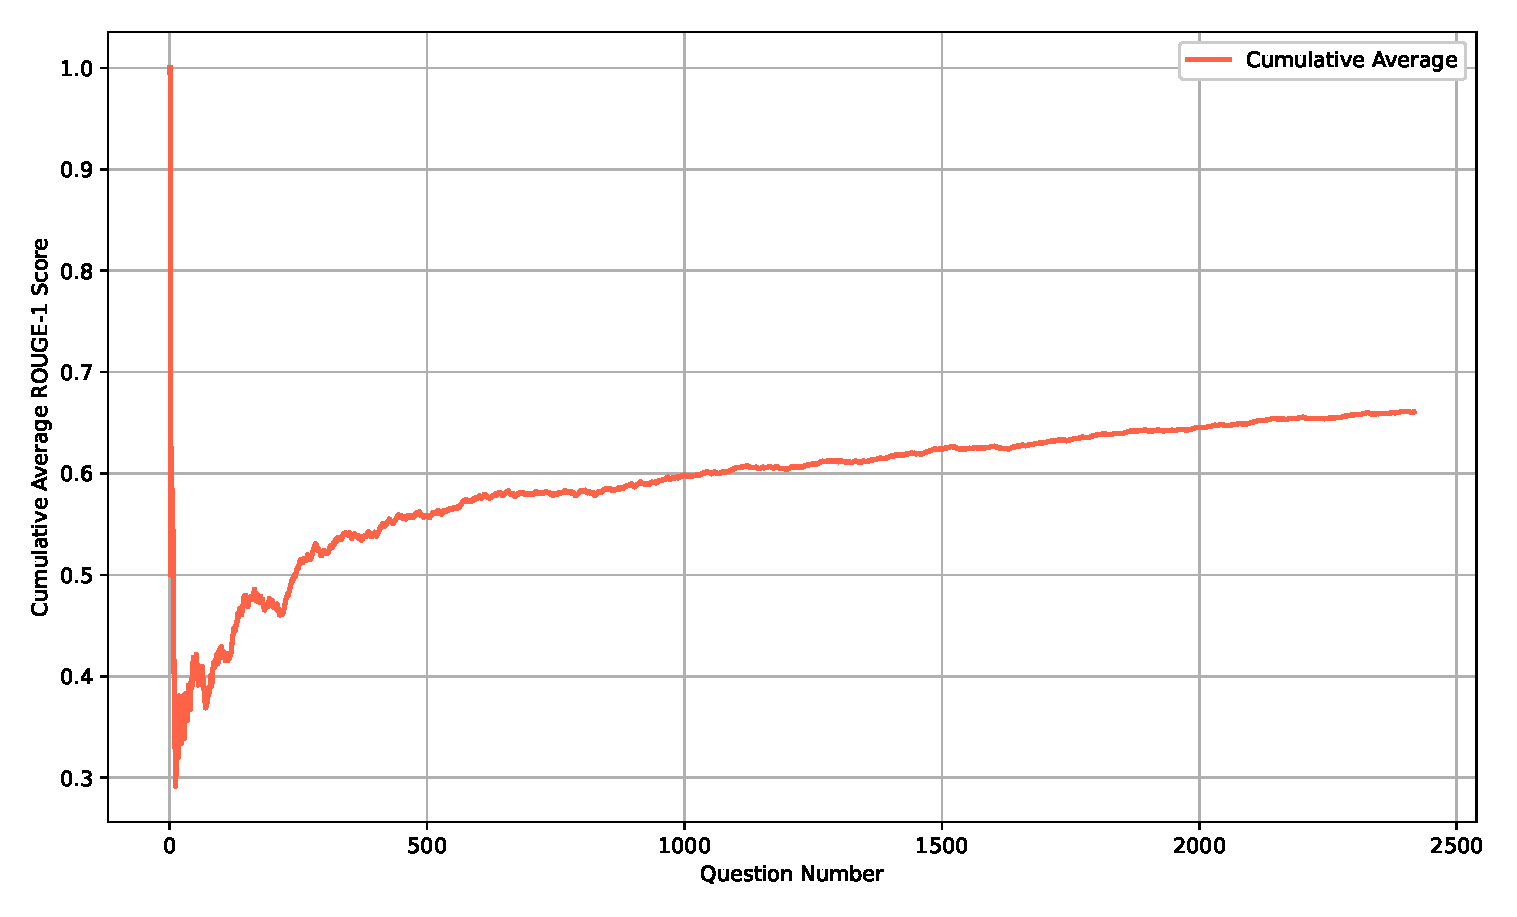
\includegraphics[width=.8\textwidth]{images/musique_cognitive_agent.eps}
    \caption{Long-lived QA Agent learning on MuSiQue using $R_1$ cumulative average.}
    \label{fig:cog_agent_learn}
\end{figure}

\noindent The Long-lived QA Agent, which incorporates episodic memory, shows pronounced gains on MuSiQue, and more moderate gains on 2Wiki. MuSiQue contains recurring question patterns and supporting evidence, enabling the agent to leverage prior experience and progressively improve over time, even with questions presented in randomized order. Figure \ref{fig:cog_agent_learn} illustrates cumulative average $R_1$ performance steadily increasing as more questions are processed. Similarly, 2Wiki contains structurally recurring questions. For example, questions such as \textit{Who is the maternal grandmother of Prince Andrew Of Greece And Denmark?}, and \textit{Who is the maternal grandmother of Archduchess Elisabeth Of Austria} follow the same pattern. Once the agent identifies how to answer such questions, it can apply similar rationale plans to new, similar questions. Recurring questions with overlapping evidence also allow previously extracted supporting information to be reused from episodic memory, facilitating more accurate responses.

\noindent To assess generalization, we evaluated the QA Agent and Long-lived QA Agent on 1,000 additional questions not included in the original evaluation sets, retrieved from the training set of each dataset. During this evaluation, the agents' memory was frozen, forcing reliance on previos learning. Results, in Table \ref{tab:qa_results_agent_v2}, show no major improvements over the baseline QA Agent, showing that this architecture only provides additional value under certain circumstances.

\begin{table}[ht]
    \centering
        \adjustbox{max width=1.1\textwidth}{
        \begin{tabular}{lcccccccccccccccc}
            \toprule
            & \multicolumn{4}{c}{\textbf{HotpotQA}} & \multicolumn{4}{c}{\textbf{2Wiki}} & \multicolumn{4}{c}{\textbf{MuSiQue}} & \multicolumn{4}{c}{\textbf{Average}} \\
            \cmidrule(lr){2-5} \cmidrule(lr){6-9} \cmidrule(lr){10-13} \cmidrule(lr){14-17}
            & EM & $R_1$ & $R_2$ & $L_1$ & EM & $R_1$ & $R_2$ & $L_1$ & EM & $R_1$ & $R_2$ & $L_1$ & EM & $R_1$ & $R_2$ & $L_1$ \\
            \midrule
            QA Agent & 70.8 & 78.4 & 44.7 & 81.0 & - & - & - & - & 46.2 & 53.6 & 31.0 & 54.0 & - & - & - & - \\
            Cognitive QA Agent & 70.4 & 78.0 & 44.1 & 80.0 & - & - & - & - & 45.7 & 53.5 & 30.6 & 54.0 & - & - & - & - \\
            \bottomrule
        \end{tabular}
        }
    \caption{\small Agents Question Answering performance on new questions.}
    \label{tab:qa_results_agent_v2}
\end{table}

\noindent We also evaluate the agents on LoCoMo. Results in Table \ref{tab:qa_results_agent_locomo}, indicate that the language agent architectures struggle to generalize to these questions. For example, the QA Agent achieves $R_1 = 47.5$, while the RAG baseline with $k = 5$ achieves $R_1 = 51.6$, despite both using GPT-4o-mini, ColBERTv2, and few-shot prompting. DAG Agent performance is similarly affected and can be counterproductive in some cases. Consider the question \textit{What is Caroline's identity?}, the RAG baseline retrieves the relevant conversation directly: 

\begin{quote}
\begin{description}[leftmargin=2em, labelwidth=3em, labelsep=0.5em, style=unboxed, font=\itshape]
    \item[Caroline:] I went to a LGBTQ support group yesterday and it was so powerful. The room was full of amazing stories and encouragement.
    \item[Melanie:] Wow, that's cool, Caroline! I'm so glad you found it.
    \item[Caroline:] The transgender stories were so inspiring! I was so happy and thankful for all the support I received there.
    \item[Melanie:] ... so cool you found such a helpful group ...
    \item[Caroline:] The support group has made me feel accepted and given me courage to embrace myself.
\end{description}
\end{quote}

\noindent From this context, it is easy to infer Caroline's identity. The DAG plan, however, begins without context and generates questions based on assumptions, such as 
\textit{What is Caroline's birthplace?} or \textit{What is Caroline's full age?}. These questions introduce bias into the reasoning process and can lead to verbose, irrelevant, or incorrect answers, demonstrating a limitation of the planning-based approach for non-compositional questions.

\begin{table}[ht]
    \centering
        \setlength{\tabcolsep}{3pt}
        \begin{tabular}{lcccc}
            \toprule
            \multicolumn{5}{c}{\textbf{LoCoMo}} \\
            \midrule
             & EM & $R_1$ & $R_2$ & $L_1$ \\
            \midrule
            \multicolumn{5}{c}{\textbf{QA Agent}} \\
            \midrule
            ColBERTv2/GPT-4o-mini & 23.3 & 47.5 & 25.2 & 43.0 \\
            ColBERTv2/GPT-4.1-mini & 17.2 & 41.2 & 21.6 & 53.0 \\
            Re-ranking (GPT-4o-mini) & 23.7 & 47.4 & 24.9 & 43.0 \\
            Pagination (GPT-4o-mini) & 24.3 & 48.8 & 25.9 & 44.0 \\
            Reflection (GPT-4o-mini) & 23.0 & 46.7 & 24.6 & 41.0 \\
            \midrule
            \multicolumn{5}{c}{\textbf{DAG Agent}} \\
            \midrule
            GPT-4o-mini & 18.8 & 41.4 & 20.2 & 37.0 \\
            GPT-4.1-mini & - & - & - & - \\
            \midrule
            \multicolumn{5}{c}{\textbf{Auto DAG Agent}} \\
            \midrule
            GPT-4o-mini & 18.4 & 39.1 & 20.0 & - \\
            GPT-4.1-mini & - & - & - & - \\
            \midrule
            \multicolumn{5}{c}{\textbf{Cognitive QA Agent}} \\
            \midrule
            GPT-4o-mini & 24.4 & 48.4 & 26.2 & 45.0 \\
            \bottomrule
        \end{tabular}
        
    \caption{Agents Question Answering performance on LoCoMo.}
    \label{tab:qa_results_agent_locomo}
\end{table}

